\section{Experiments}

\againframe{Motivation}
% Difficult to model the magnetosphere over an 11 year cycle today, GEM
% challenge is only 6-8 events, each event is unique, documenting the tendencies
% of models gives a reference to model developers as to why a model does poorly

\againframe{Experiments}

\subsection{$B_z$ Reversal}
\begin{frame}
	\frametitle{Experiment Setup}
	\begin{itemize}
 	 \item $B_z$ reversal from positive to negative at 00:30 out of 06:00. 
 	 \item Other input variables kept at 11 year means.
 	\begin{table}
 	\small
	\begin{center}
  	\caption{Chosen values for CCMC run 1}
  	\begin{tabular}{| l | c | c | c | c | }
    \hline
    \textbf{Run Num.} & \textbf{$\rho$} [$cm^{-3}$] & \textbf{$T$} [$K$] &
    \textbf{$U_x$} [$km/s$] &
    \textbf{$B_z$} [$nT$]
    \\
    \hline 
    1 & 5.76 & 101289 & -442  & +3.1 to -3.0 at 00:30 \\ \hline
  \end{tabular}
  \label{table:runs12}
\end{center}
\end{table}
	\begin{figure}
		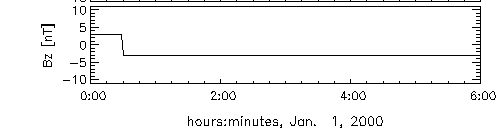
\includegraphics[scale=0.3]{images/CCMCRun1.png}
		\caption{CCMC run 1 plot of input time series }
	\end{figure}
	\end{itemize}
\end{frame}

\begin{frame}
	\frametitle{Input Variable Selection}\
	\begin{figure}
		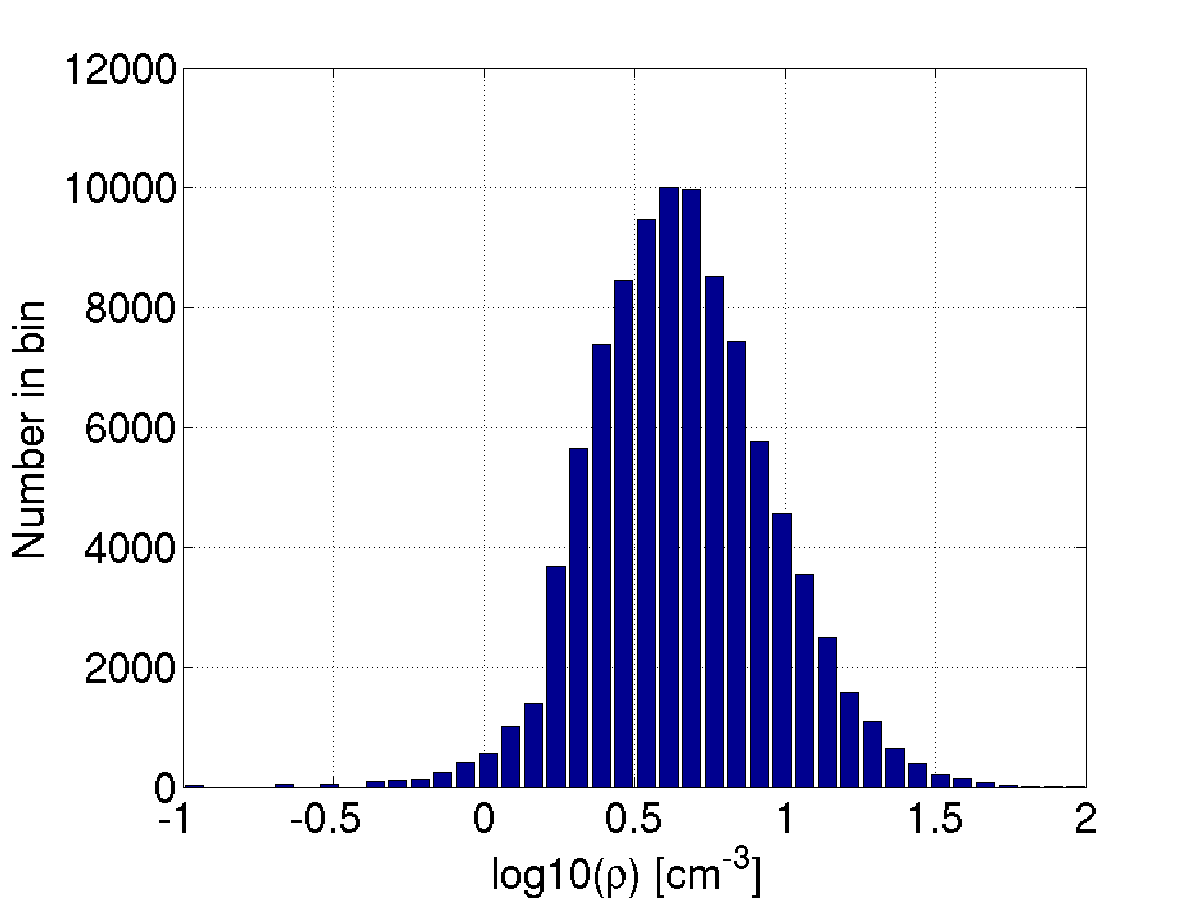
\includegraphics[scale=0.17]{images/hist_N.png}\quad
		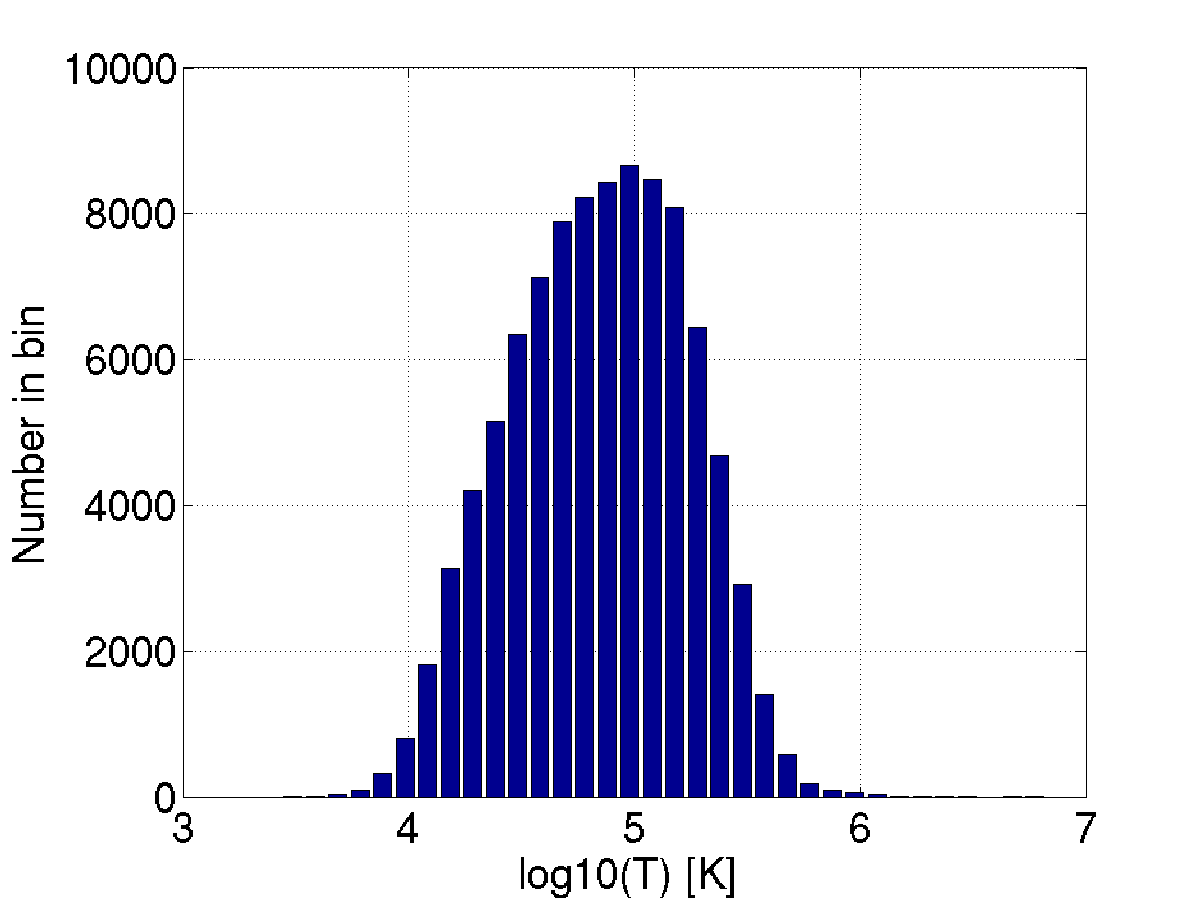
\includegraphics[scale=0.17]{images/hist_T.png}\\
		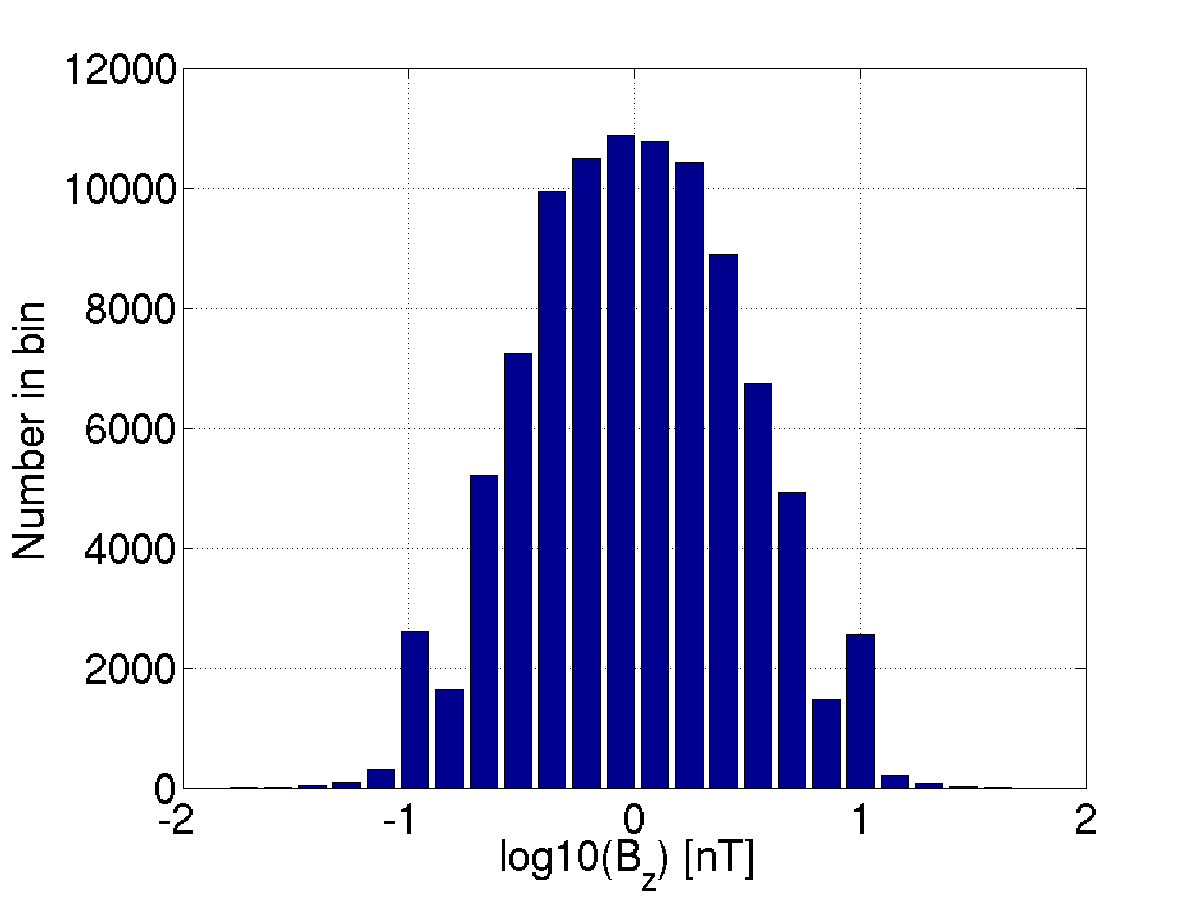
\includegraphics[scale=0.17]{images/hist_BZ.png}\quad
		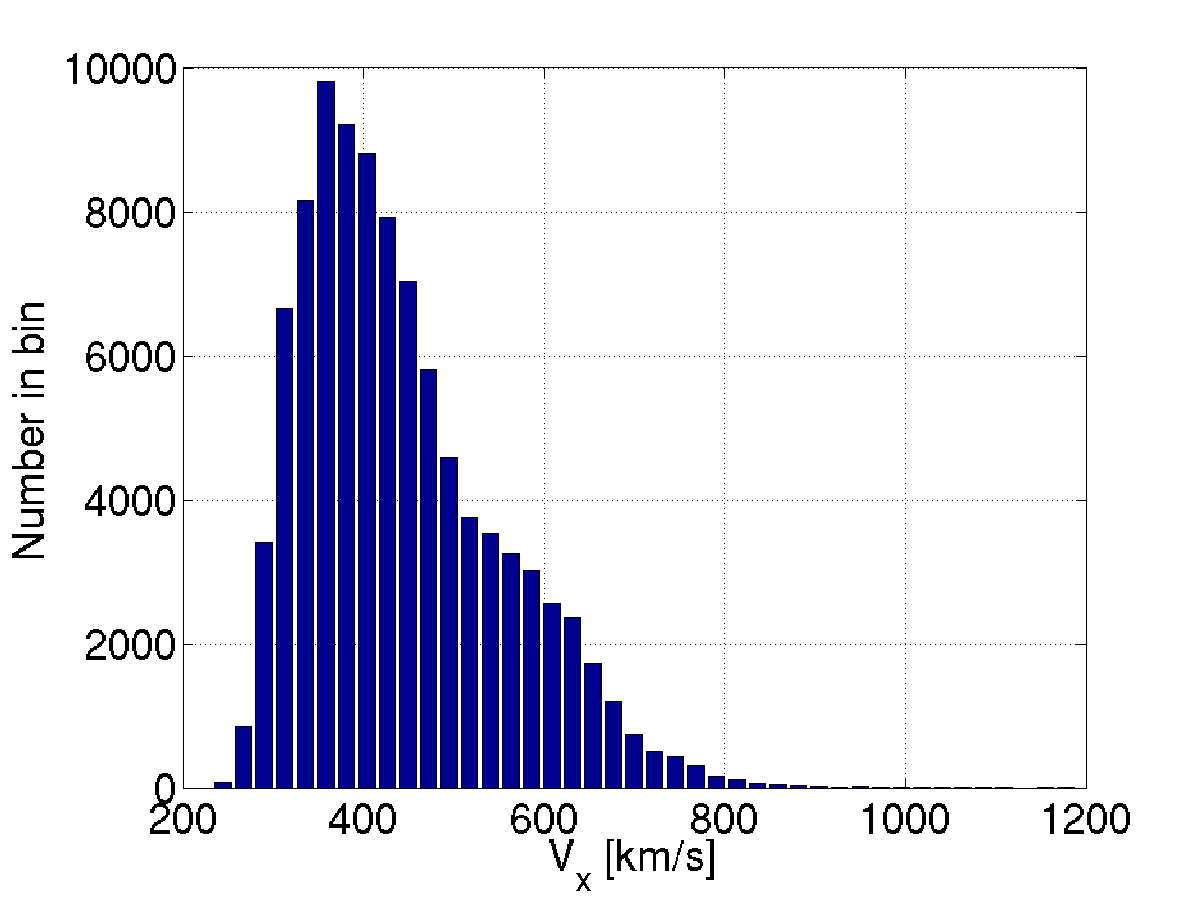
\includegraphics[scale=0.17]{images/hist_V.png}\\
		\caption{Jan 1, 2000 to Jan 1, 2011 Histograms of ACE Data }
\end{figure}
\end{frame}

\begin{frame}
\frametitle{$B_z$ Analysis: Magnetopause locations}
\begin{itemize}
  \item Important for satellite operations. Avoid crossing from magnetosphere
  into solar wind.
  \item For this experiment:
  \begin{itemize}
    \item No ring current and northward IMF $B_z$
    \item No ring current and southward IMF $B_z$
    \item Included ring current and northward IMF $B_z$
    \item Included ring current and southward IMF $B_z$
  \end{itemize}
\end{itemize}
\end{frame}

\begin{frame}
	\frametitle{No ring current and northward IMF $B_z$}
	\begin{columns}
	\begin{column}{.6\textwidth}
	\begin{figure}
		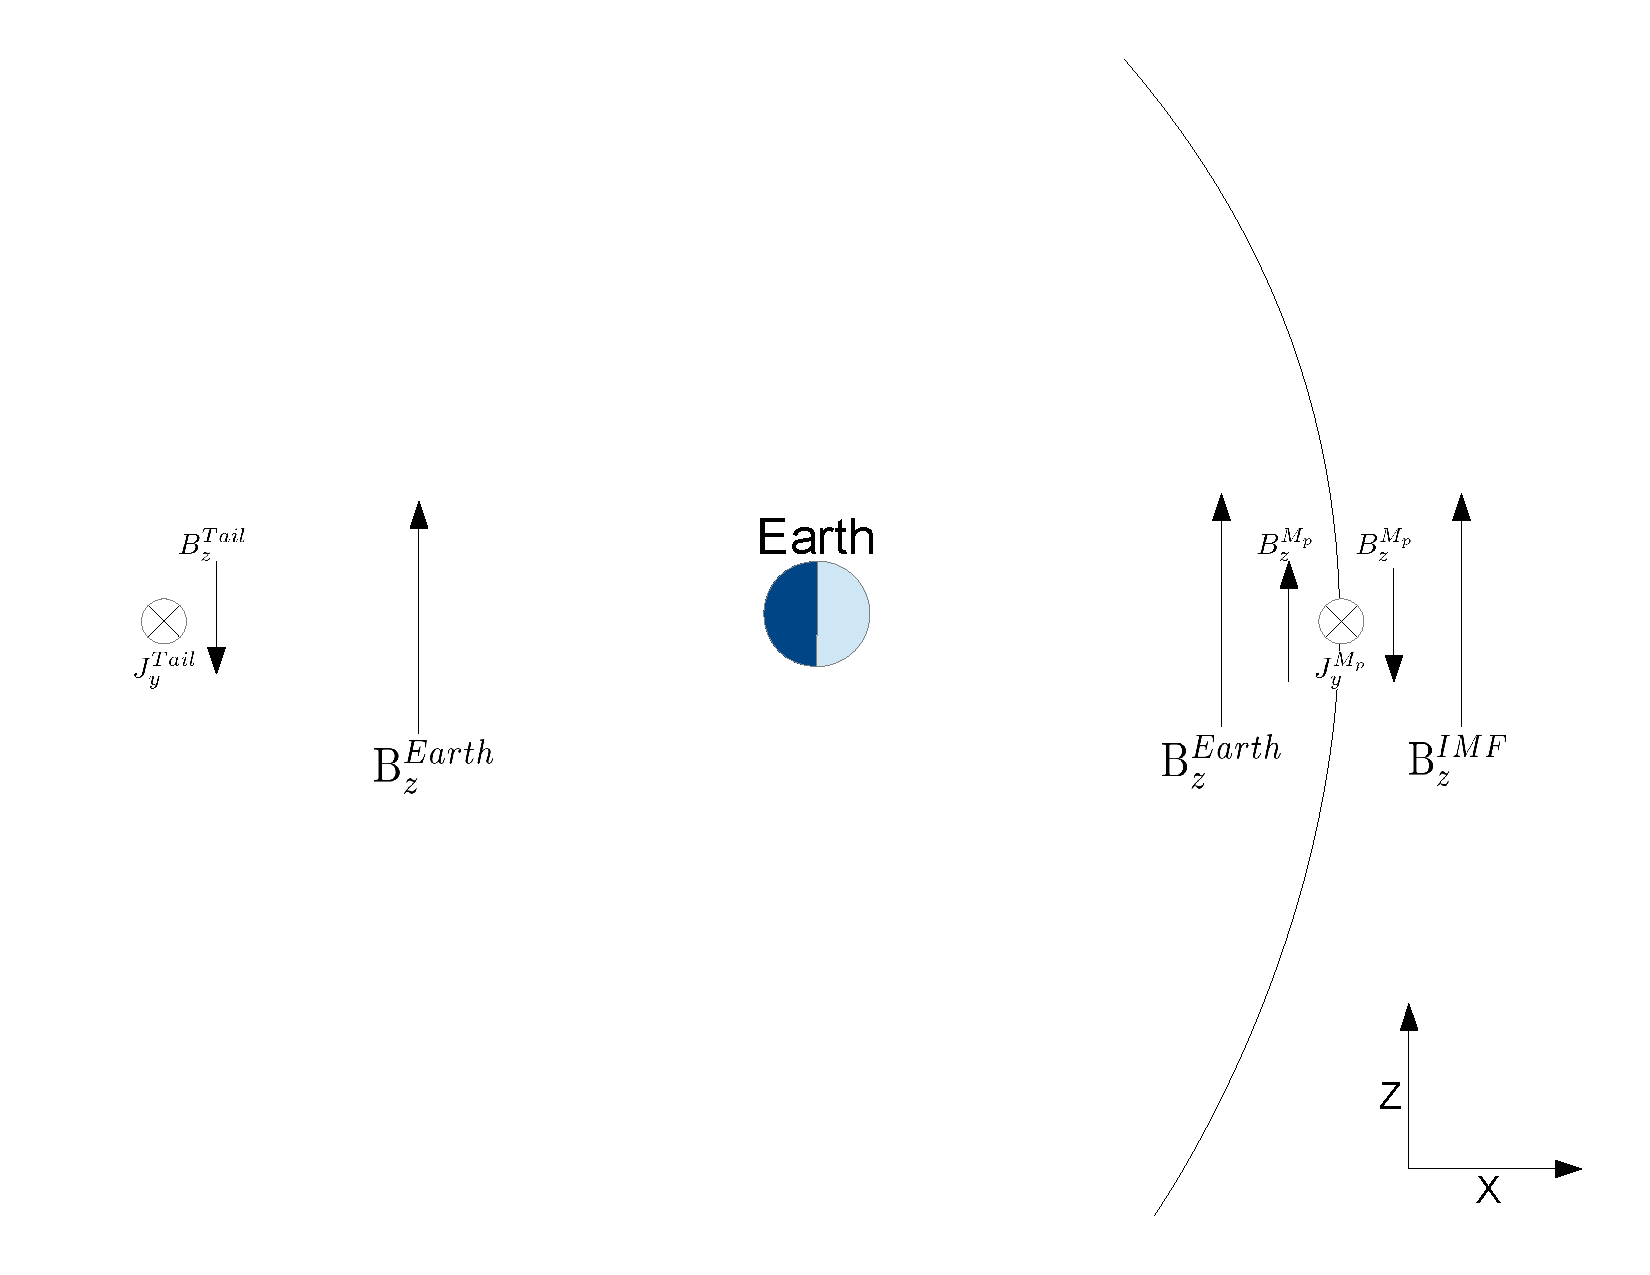
\includegraphics[scale=.23]{images/NimfNoRC.pdf}
	\end{figure}
	\end{column}
	\begin{column}{.4\textwidth}
	\begin{figure}
		\textbf{BATS-R-US $B_z$}\\
		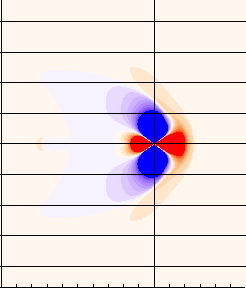
\includegraphics[scale=.45]{images/NBzNoRCM.png}
	\end{figure}
	\end{column}
	\end{columns}
\end{frame}

\begin{frame}
	\frametitle{No ring current and southward IMF $B_z$}
	\begin{columns}
	\begin{column}{.6\textwidth}
	\begin{figure}
		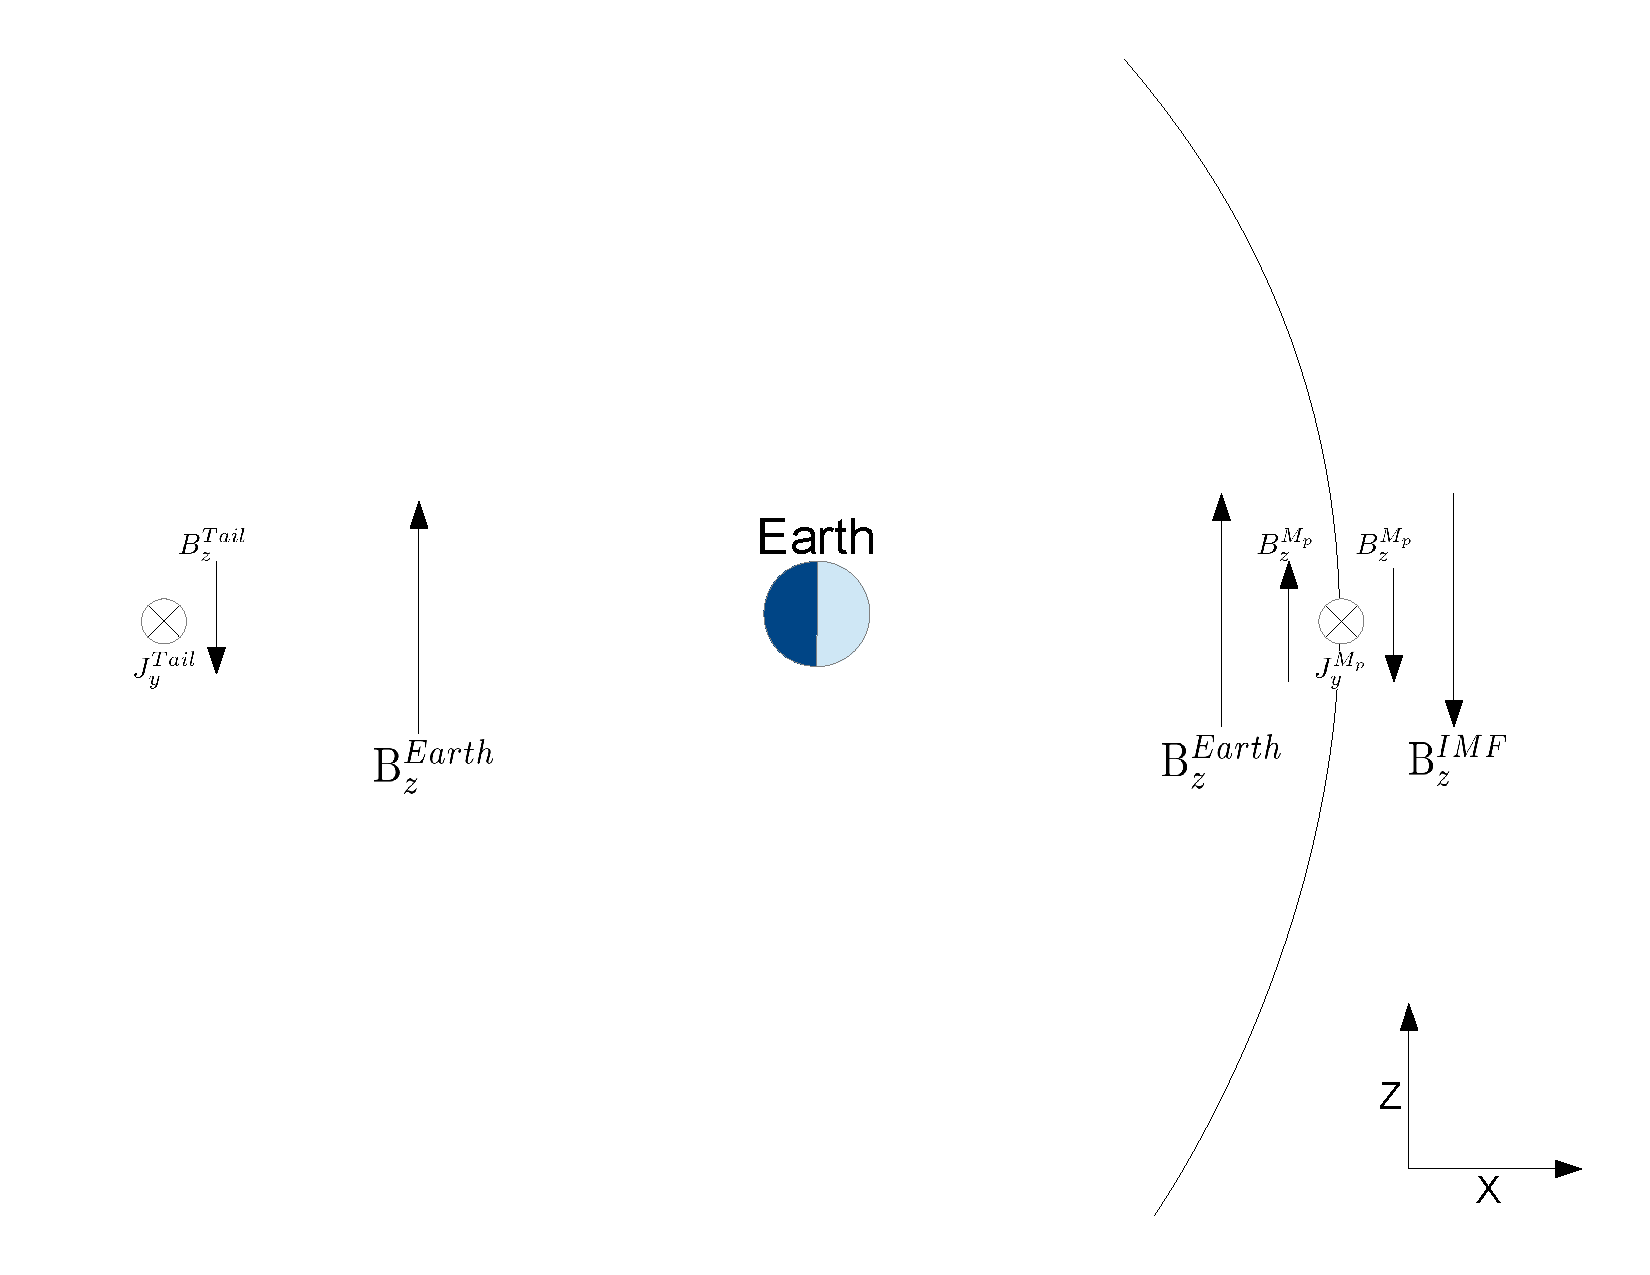
\includegraphics[scale=.23]{images/SimfNoRC.pdf}
	\end{figure}
	\end{column}
	\begin{column}{.4\textwidth}
	\begin{figure}
	\textbf{BATS-R-US $B_z$}\\
	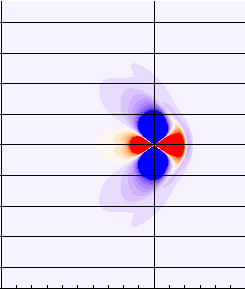
\includegraphics[scale=.45]{images/SBzNoRCM.png}
	\end{figure}
	\end{column}
	\end{columns}
\end{frame}

\begin{frame}
	\frametitle{Included ring current and northward IMF $B_z$}
	\begin{columns}
	\begin{column}{.6\textwidth}
	\begin{figure}
		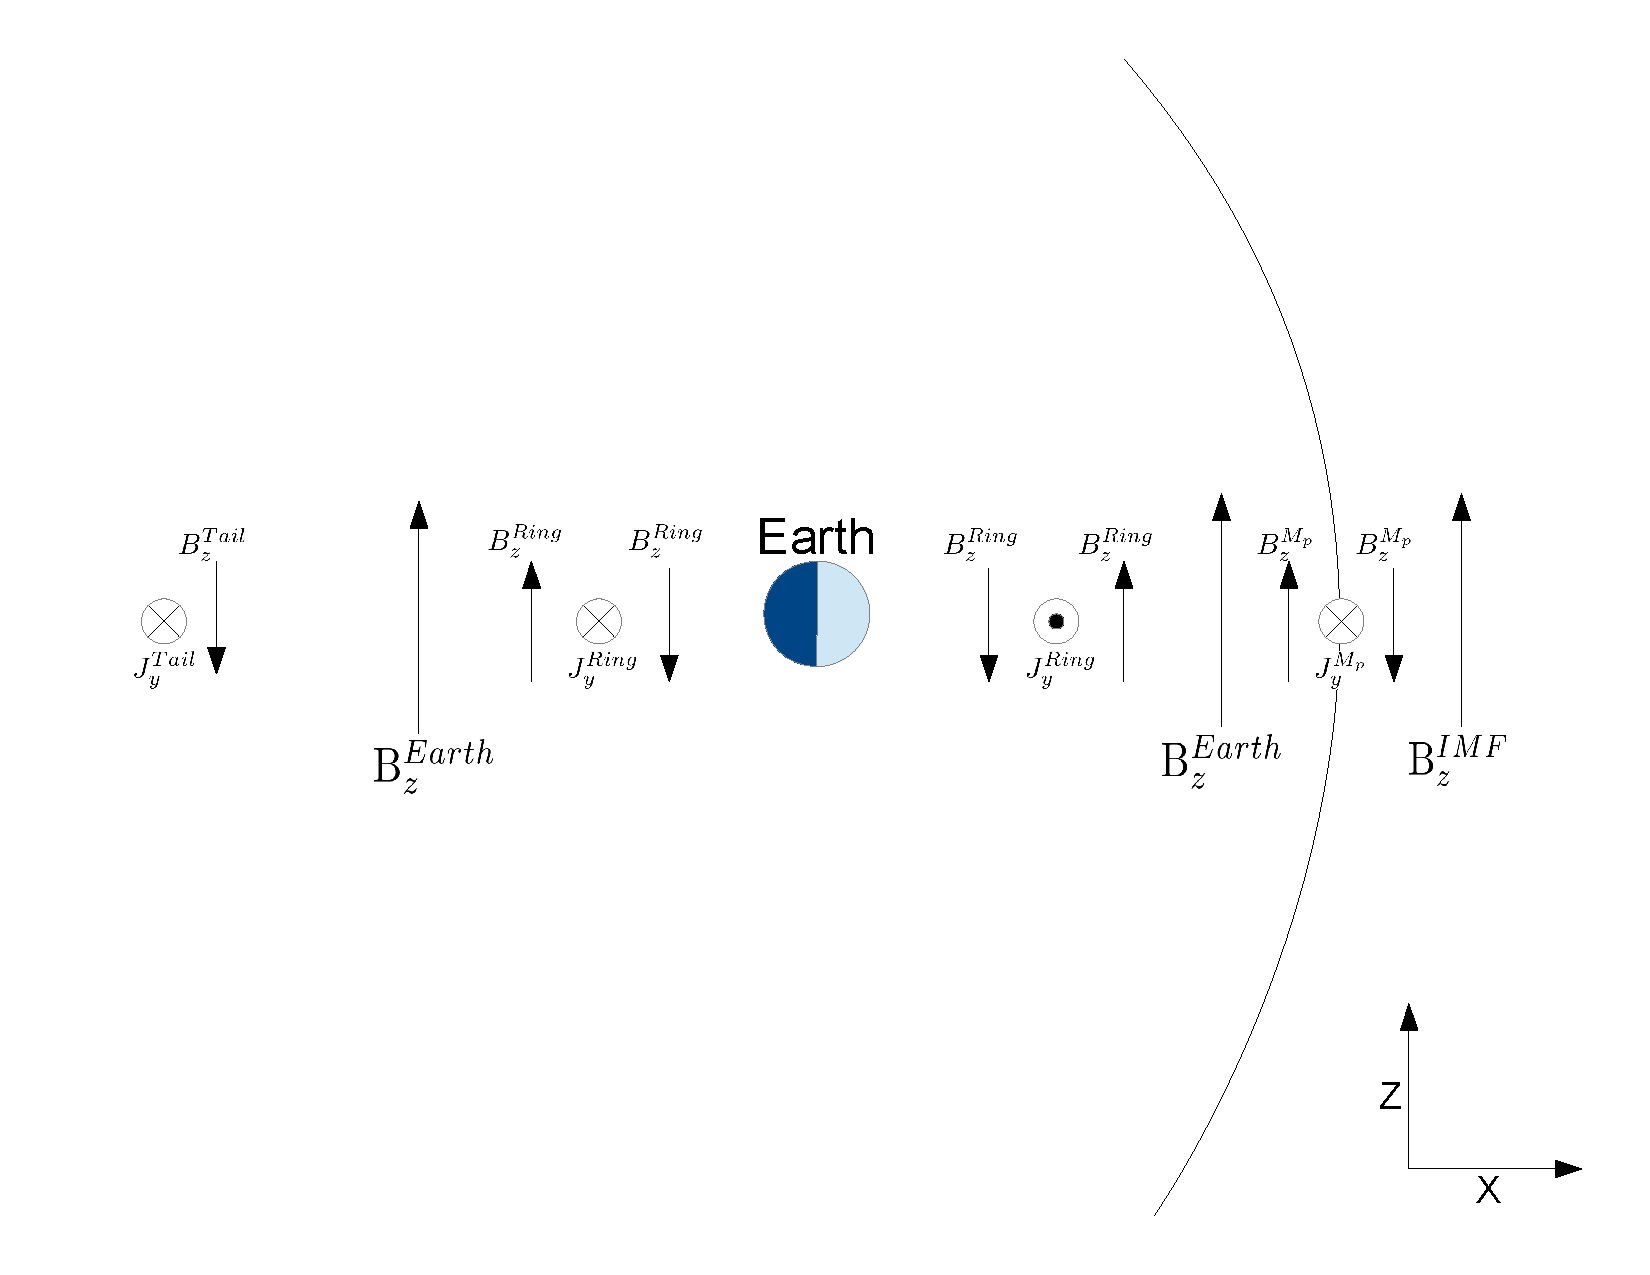
\includegraphics[scale=.23]{images/NimfRC.pdf}
		
	\end{figure}
	\end{column}
	\begin{column}{.4\textwidth}
	\begin{figure}
		\textbf{SWMF $B_z$}\\
		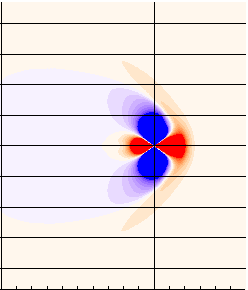
\includegraphics[scale=.45]{images/NBzRCM.png}
	\end{figure}
	\end{column}
	\end{columns}
\end{frame}

\begin{frame}
	\frametitle{Included ring current and southward IMF $B_z$}
	\begin{columns}
	\begin{column}{.6\textwidth}
	\begin{figure}
		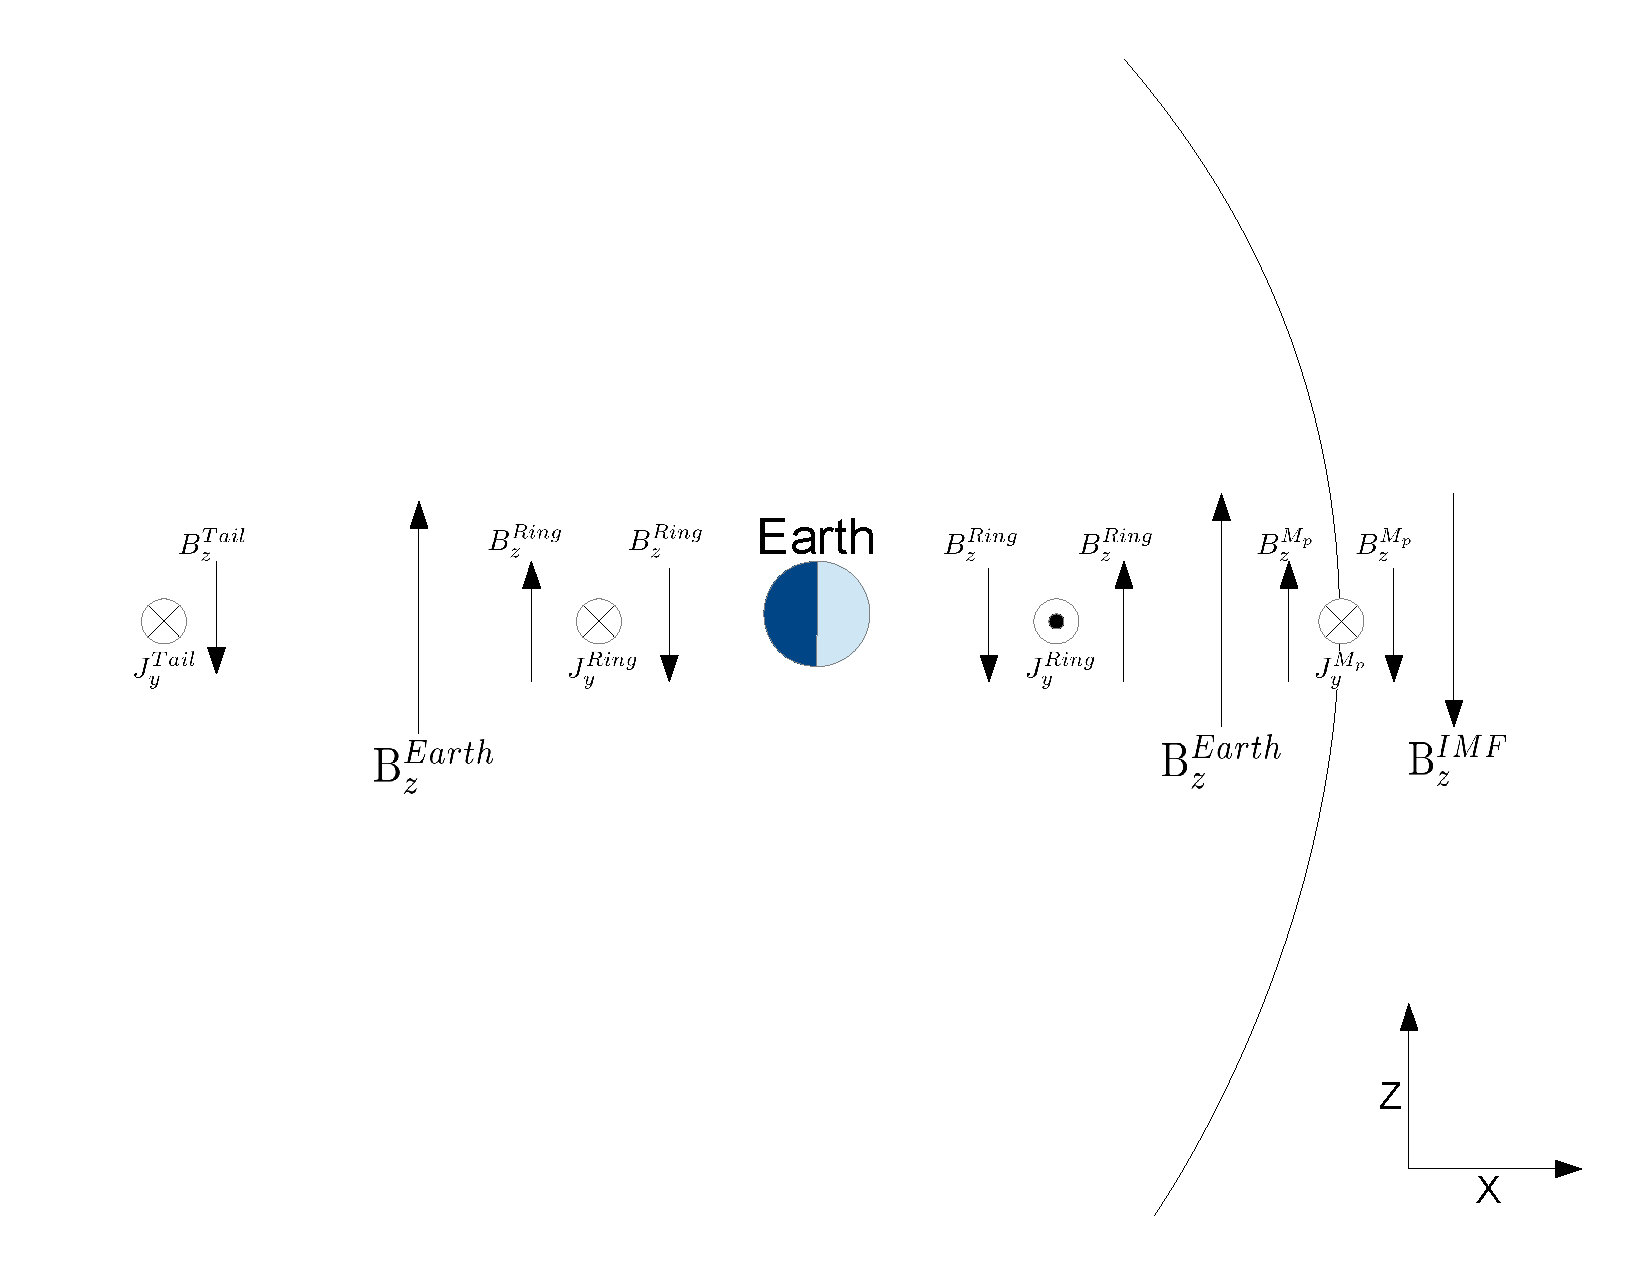
\includegraphics[scale=.23]{images/SimfRC.pdf}
	\end{figure}
	\end{column}
	\begin{column}{.4\textwidth}
	\begin{figure}
		\textbf{SWMF $B_z$}\\
		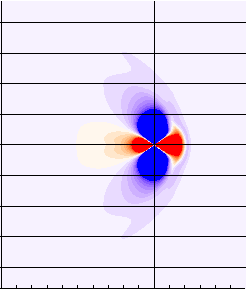
\includegraphics[scale=.45]{images/SBzRCM.png}
	\end{figure}
	\end{column}
	\end{columns}
\end{frame}

\begin{frame}
\frametitle{$B_z$ Differences}
\begin{center}
\begin{figure}
\includegraphics[scale=0.15]{/mnt/Disk2/Brian_Curtis_042213_1/Results/images/Bz_File5.png}\\
\includegraphics[scale=0.15]{/mnt/Disk2/Brian_Curtis_042213_2/Results/images/Bz_File5.png}\\
\caption{OpenGGCM (top) and BATS-R-US (bottom) northward IMF $B_z$}
\end{figure}
\end{center}
\end{frame}


\begin{frame}
\frametitle{$B_z$ Differences}
\begin{center}
\begin{figure}
\href{images/1_ReversalB.pdf}{\includegraphics[scale=0.3]{/mnt/Disk2/Results/0_1/images/Bz_Diff_File5.png}}\\
\caption{OpenGGCM - BATS-R-US $B_z$ Percent Diff }
\end{figure}
\end{center}
\end{frame}

\begin{frame}
\frametitle{$B_z$ Differences}
\begin{center}
\begin{figure}
\includegraphics[scale=0.15]{/mnt/Disk2/Results/0_2/images/Bz_Diff_File5.png}\\
\includegraphics[scale=0.15]{/mnt/Disk2/Results/1_2/images/Bz_Diff_File5.png}\\
\caption{OpenGGCM - SWMF (top) and BATS-R-US - SWMF (bottom) northward IMF
$B_z$ differences}
\end{figure}
\end{center}
\end{frame}

\begin{frame}
\frametitle{$B_z$ Differences}
\begin{center}
\begin{figure}
\includegraphics[scale=0.15]{/mnt/Disk2/Results/0_2/images/Bz_Diff_File30.png}\\
\includegraphics[scale=0.15]{/mnt/Disk2/Results/1_2/images/Bz_Diff_File30.png}\\
\caption{OpenGGCM - SWMF (top) and BATS-R-US - SWMF (bottom) southward IMF
$B_z$ differences}
\end{figure}
\end{center}
\end{frame}

\begin{frame}
\frametitle{$\rho$ Differences}
\begin{center}
\begin{figure}
\includegraphics[scale=0.15]{/mnt/Disk2/Brian_Curtis_042213_1/Results/images/rho_File5.png}\\
\includegraphics[scale=0.15]{/mnt/Disk2/Brian_Curtis_042213_3/Results/images/rho_File5.png}\\
\caption{OpenGGCM (top) and SWMF (bottom) $\rho$}
\end{figure}
\end{center}
\end{frame}


\begin{frame}
\frametitle{$\rho$ Differences}
\begin{center}
\begin{figure}
\includegraphics[scale=0.3]{/mnt/Disk2/Results/0_2/images/rho_Diff_File5.png}\\
\caption{OpenGGCM - SWMF $\rho$ Percent Diff}
\end{figure}
\end{center}
\end{frame}

\begin{frame}
\frametitle{Expected $U_x$}
\begin{figure}
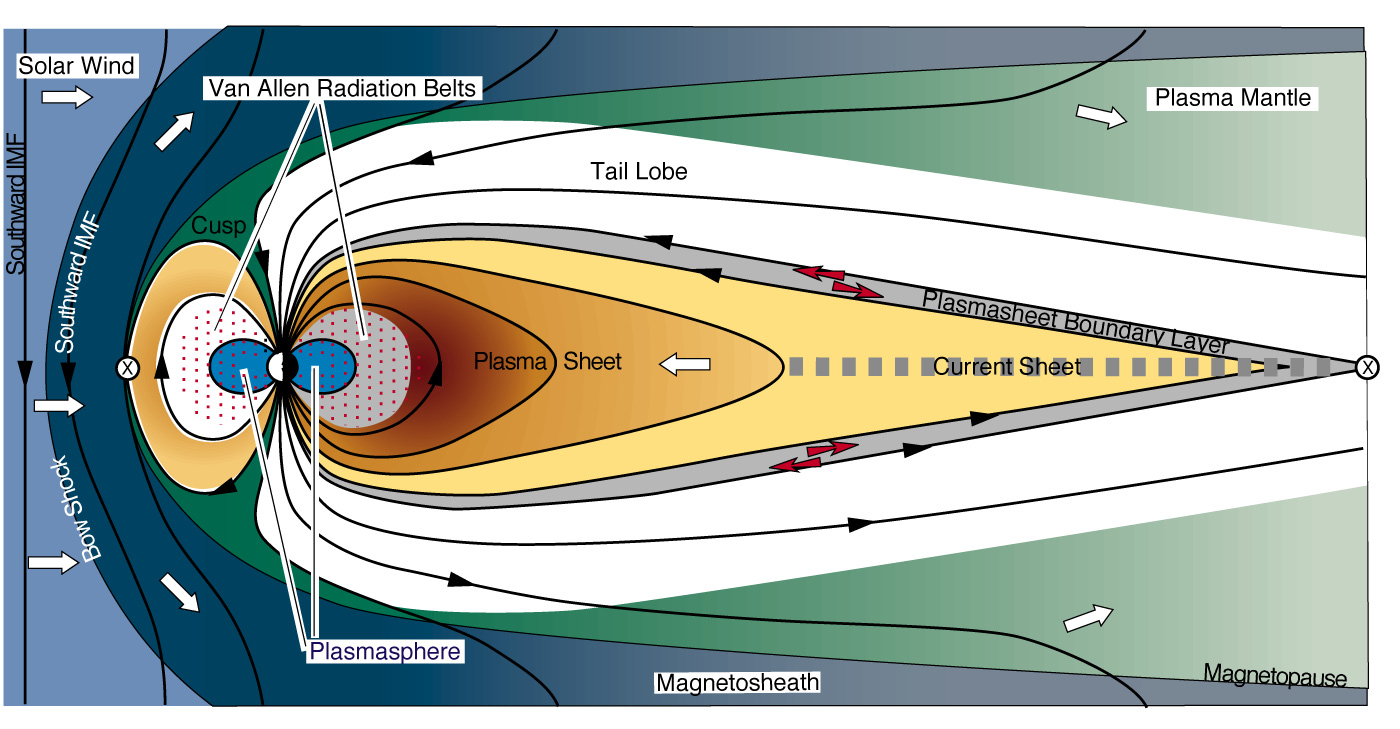
\includegraphics[scale=0.21]{images/Rice_Magnetosphere.jpg}\\
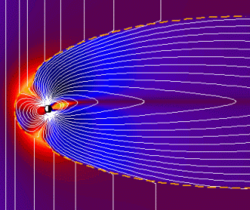
\includegraphics[scale=0.4]{images/tsyganenko.png}
\end{figure}
\end{frame}

\begin{frame}
\frametitle{$U_x$ Plots}
\begin{center}
\begin{figure}
\includegraphics[scale=0.15]{/mnt/Disk2/Brian_Curtis_042213_2/Results/images/Ux_File5.png}\\
\includegraphics[scale=0.15]{/mnt/Disk2/Brian_Curtis_042213_3/Results/images/Ux_File5.png}\\
\caption{BATS-R-US (top) and SWMF (bottom) $U_x$}
\end{figure}

\end{center}
\end{frame}


\begin{frame}
\frametitle{$U_x$ Differences}
\begin{center}
\begin{figure}
\includegraphics[scale=0.3]{/mnt/Disk2/Results/1_2/images/Ux_Diff_File5.png}\\
\caption{BATS-R-US - SWMF $U_x$ Percent Diff}
\end{figure}
\end{center}
\end{frame}

\begin{frame}[shrink]
\frametitle{$B_z$ Reversal Conclusions}
For a reversal in IMF $B_z$, the following occur in the models:
\begin{itemize}
  \item The OpenGGCM magnetopause is closest to Earth as it has the weakest
  magnetic pressure near-Earth.
  \item In positive IMF $B_z$ conditions, the ring current pushes the SWMF
  magnetopause farther Sunward than the BATS-R-US.
  \item In negative IMF $B_z$ conditions, the SWMF magnetopause is farther
  Earthward than the BATS-R-US.
  \item The differences in magnetopause positions between the BATS-R-US and SWMF
  are due to the effects of the ring current addition to the magnetosphere in
  the SWMF model.
  \item Densities are highest with the SWMF and lowest with the OpenGGCM.
  \item The OpenGGCM tail velocities are largely different from the BATS-R-US
  and SWMF.
\end{itemize}
\end{frame}

\subsection{Preconditioning}

\begin{frame}
\frametitle{Preconditioning Definition}
\textbf{Definition:} Magnetospheric model pre-conditioning takes an
initial state, then the model is iterated through time and conditions are slowly
changed to meet the initial conditions set by the user.
\begin{itemize}
  \item Earth's magnetic field is set as a dipole, mirror dipole at ~16$R_e$. Plasma temperature and density initially set to 5000 [$K$] and 0.1
  [$cm^{-3}$] respectively.
  \item OpenGGCM: Uses 2 hours of preconditioning that includes 30 minutes with
  negative Bz.
  \item BATS-R-US/SWMF: Uses a local time stepping scheme where an approximate
  steady state is reached after 2500 iteration steps.
\end{itemize}
\end{frame}

\begin{frame}[shrink]
\frametitle{Experiment Setup}
\begin{itemize}
  \item First run: $B_z$ reversal at 00:30 (early reversal)
  \item Second run: Delay $B_z$ reversal until 02:00 (late reversal)
  \item Take equal data sample sizes matching the reversal times.
  \item Compare models with themselves at two different reversal times.
\end{itemize}
\end{frame}

\begin{frame}
\frametitle{Model Outputs}
\begin{tabular}{p{0.4\textwidth}p{0.5\textwidth}}
\begin{itemize}
  \item[]
  \includegraphics[scale=0.10]{/mnt/Disk2/Precondition/Results/0_3/images/Ux_Diff_File5.png}
  \item[]
  \includegraphics[scale=0.10]{/mnt/Disk2/Precondition/Results/1_4/images/Ux_Diff_File5.png}
  \item[]
  \includegraphics[scale=0.10]{/mnt/Disk2/Precondition/Results/2_5/images/Ux_Diff_File5.png}
\end{itemize}
 &
\begin{itemize}
  \setlength{\itemsep}{43pt}
  \item \href{images/2_PreconditionOpenGGCM.pdf}{OpenGGCM}
  \item \href{images/3_PreconditionBATSRUS.pdf}{BATS-R-US}
  \item \href{images/4_PreconditionSWMF.pdf}{SWMF}
\end{itemize}
\end{tabular}
\end{frame}

\begin{frame}[shrink]
\frametitle{Preconditioning Conclusions}
For changes in the preconditioning time of magnetospheric MHD models the
following shows that there is a significant sensitivity to preconditioning time
and supports that there is a need for a more detailed analysis:
\begin{itemize}
  \item Longer preconditioning time allowed the magnetosphere to relax more
  giving different positions for the magnetopause with all three models.
  \item The OpenGGCM magnetopause position differences were wider than that of
  SWMF or BATS-R-US.
  \item There were large differences for all three models before the $B_z$
  reversal.
  \item The differences in the current sheet region for the OpenGGCM were
  similar before and after the reversal.
  \item The BATS-R-US and SWMF differences decreased after the $B_z$ reversal to
  near zero.
\end{itemize}
\end{frame}

\subsection{Extreme Conditions}

\begin{frame}
\frametitle{Experiment Setup}
\begin{table}
\begin{center}
  \caption{Chosen values for CCMC runs 3 and 4}
  \begin{tabular}{| l | c | c | c | c | }
    \hline
    \textbf{Run Num.} & \textbf{$\rho$} & \textbf{$T$} & \textbf{$Vx$} &
    \textbf{$B_z$}
    \\
    \hline 
    3 & 11 & 101289 & -604  & -3.0 \\ \hline
    4 & 2 & 101289 & -320  & 3.1 \\ \hline
  \end{tabular}
  \label{table:runs34}
\end{center}
\end{table}
\begin{tabular}{p{0.5\textwidth}p{0.5\textwidth}}
\begin{itemize}
  \item[]\includegraphics[scale=0.12]{/mnt/Disk2/Brian_Curtis_042413_1/Results/images/Bz_File5.png}\\
  \item[] Run 3 - High Compression
\end{itemize}
 &
\begin{itemize}
  \item[]\includegraphics[scale=0.12]{/mnt/Disk2/Brian_Curtis_042413_5/Results/images/Bz_File5.png}\\
  \item[] Run 4 - Low Compression
\end{itemize}
\end{tabular}
\end{frame}

\begin{frame}
\frametitle{Low Compression - Model Output}
\begin{columns}
\begin{column}{.33\textwidth}
\begin{figure}
	\textbf{$B_z$ Percent Diff}\\
	\includegraphics[scale=0.10]{/mnt/Disk2/Results/0_1/images/Bz_Diff_File5.png}\\
  	\includegraphics[scale=0.10]{/mnt/Disk2/Results/0_2/images/Bz_Diff_File5.png}\\
  	\includegraphics[scale=0.10]{/mnt/Disk2/Results/1_2/images/Bz_Diff_File5.png}
\end{figure}
\end{column}
&
\begin{column}{.33\textwidth}
\begin{figure}
	\textbf{$\rho$ Percent Diff}\\
	\includegraphics[scale=0.10]{/mnt/Disk2/Results/0_1/images/rho_Diff_File5.png}\\
  	\includegraphics[scale=0.10]{/mnt/Disk2/Results/0_2/images/rho_Diff_File5.png}\\
  	\includegraphics[scale=0.10]{/mnt/Disk2/Results/1_2/images/rho_Diff_File5.png}
\end{figure}
\end{column}
&
\begin{column}{.33\textwidth}
\begin{figure}
	\textbf{$U_x$ Percent Diff}\\
	\includegraphics[scale=0.10]{/mnt/Disk2/Results/0_1/images/Ux_Diff_File5.png}\\
  	\includegraphics[scale=0.10]{/mnt/Disk2/Results/0_2/images/Ux_Diff_File5.png}\\
  	\includegraphics[scale=0.10]{/mnt/Disk2/Results/1_2/images/Ux_Diff_File5.png}
\end{figure}
\end{column}
\end{columns}
\end{frame}

\begin{frame}
\frametitle{High Compression - Model Output}
\begin{tabular}{p{0.4\textwidth}p{0.5\textwidth}}
\begin{itemize}
  \item[]
  \includegraphics[scale=0.10]{/mnt/Disk2/Brian_Curtis_042413_1/Results/images/Ux_File5.png}
  \item[]
  \includegraphics[scale=0.10]{/mnt/Disk2/Brian_Curtis_042413_2/Results/images/Ux_File5.png}
  \item[]
  \includegraphics[scale=0.10]{/mnt/Disk2/Brian_Curtis_042413_3/Results/images/Ux_File5.png}
\end{itemize}
 &
\begin{itemize}
  \setlength{\itemsep}{43pt}
  \item \href{images/5_HighOpenGGCM.pdf}{OpenGGCM}
  \item \href{images/6_HighBATSRUS.pdf}{BATS-R-US}
  \item \href{images/7_HighSWMF.pdf}{SWMF}
\end{itemize}
\end{tabular}
\end{frame}

\begin{frame}[shrink]
\frametitle{Extreme Conditions Conclusions}
For extreme conditions in the solar wind, the
following occurs in the magnetosphere:
\begin{itemize}
  \item The OpenGGCM has a large region of Earthward $U_x$ in the current sheet
  region that grows as time progresses in a compressed environment.
  \item The BATS-R-US is either completely stable or stops in a compressed
  environment.
  \item In a compressed environment the SWMF will eventually oscillate.
  \item The OpenGGCM has the highest tailward velocities in a compressed
  environment.
  \item The ring current reduced the maximum velocities in the SWMF.
  \item The OpenGGCM has the highest $B_z$ in a compressed environment.
  \item All three models have similar magnetopause positions in a low
  compression environment.
  \item The OpenGGCM current sheet velocities are largest in a low compression
  environment.
\end{itemize}
\end{frame}
